\documentclass[10pt,conference]{IEEEtran}

\usepackage[T1]{fontenc}
\usepackage[utf8]{inputenc}
\usepackage{lmodern}
\usepackage{microtype}
\usepackage{amsmath}
\usepackage{booktabs}
\usepackage{graphicx}
\usepackage[hidelinks]{hyperref}
\usepackage[numbers]{natbib}

\title{Provider-Dependent Reliability of Self-Reported Confidence under a Shared Black-Box MT Protocol}
\author{\IEEEauthorblockN{Umberto Altieri}}

\begin{document}
\maketitle

\begin{abstract}
This paper evaluates a trustworthy-AI reliability question for black-box language-model services: whether one confidence threshold can be reused across providers under a shared protocol. We run eight models from OpenAI, Anthropic, and Google on 500 WMT17 English$\rightarrow$German sentences (4,000 translation--confidence pairs), with sentence-level chrF and an operational low-quality target (within-model bottom 20\%). Despite similar mean chrF (54.0--60.1), provider reliability differs sharply: ECE spans 0.076--0.180 and mismatch@0.9 spans 0.2\%--18.2\%. The released snapshot also shows uneven parse-warning burden (443/4000 rows; 11.1\%), which is an implementation-level confound. The supported conclusion is narrow: under this protocol and target, self-reported confidence is not portable as a shared probability scale, so common thresholds do not yield comparable routing/abstention operating points. We also report conservative limitations: no bundled COMET/xCOMET checkpoints, no completed semantic-audit labels, and no bundled non-baseline prompt-variant outputs.
\end{abstract}

\section{Introduction}
Confidence-guided routing and abstention policies are increasingly used in AI-assisted workflows, but they often assume that scores from different providers are comparable on a common scale. This paper tests that assumption in a controlled black-box setting. We use the same prompt protocol and JSON schema across providers, collect translation and post-hoc self-reported confidence, and evaluate reliability against a reproducible operational target.

Our framing is trustworthy AI rather than generic MT quality: if identical threshold policies induce materially different failure rates across providers, confidence cannot be treated as a portable control signal. This matters for safe decision support pipelines that switch or combine providers.

\section{Setup and Metrics}
\textbf{Data and models.} We use 500 WMT17 \texttt{en-de} sentences (seed 123), eight models across three providers, and temperature 0. This yields 4,000 outputs.

\textbf{Protocol.} Each input gets a translation call and a confidence call, both strict JSON. Prompts are rendered from shared templates; provider adapters handle transport.

\textbf{Operational target.} Low quality is defined as the within-model bottom 20\% by sentence chrF. The study is therefore about alignment to an operational overlap-based event, not semantic correctness calibration.

\textbf{Primary diagnostics.} We report ECE (10 bins) and mismatch@0.9, where mismatch is
\[
\Pr(\text{low-quality} \wedge \text{confidence}>0.9).
\]

\section{Main Results}
Table~\ref{tab:main} is the core evidence. Mean chrF is relatively close across models, but ECE and mismatch@0.9 vary widely. This implies that a shared threshold (e.g., 0.9) induces provider-specific operating points.

\begin{table}[t]
\centering
\small
\begin{tabular}{lcccc}
\toprule
Model & Mean chrF & ECE (within-q20) & Mismatch@0.9 & Median conf. \\
\midrule
anthropic/claude-haiku-4-5-20251001 & 57.01 & 0.094 & 13.4\% & 0.92 \\
anthropic/claude-opus-4-6 & 58.45 & 0.087 & 7.6\% & 0.93 \\
anthropic/claude-sonnet-4-5-20250929 & 56.89 & 0.095 & 12.8\% & 0.95 \\
gemini/gemini-2.5-flash & 54.01 & 0.148 & 4.2\% & 0.73 \\
gemini/gemini-2.5-pro & 60.07 & 0.180 & 18.2\% & 1.00 \\
openai/gpt-5-mini & 57.09 & 0.152 & 12.8\% & 0.93 \\
openai/gpt-5-nano & 55.31 & 0.076 & 0.2\% & 0.73 \\
openai/gpt-5.2 & 58.87 & 0.134 & 15.2\% & 0.93 \\
\bottomrule
\end{tabular}
\caption{Main summary table from regenerated code-side outputs (within-model chrF-q20 target).}
\label{tab:main}
\end{table}


Figure~\ref{fig:reliability} provides a qualitative reliability view; Figure~\ref{fig:mismatch} shows stratified mismatch by source-side complexity quartiles. The quartile view is secondary and descriptive only.

\begin{figure}[t]
\centering
\IfFileExists{figures/fig2_reliability_diagram_overlay.pdf}{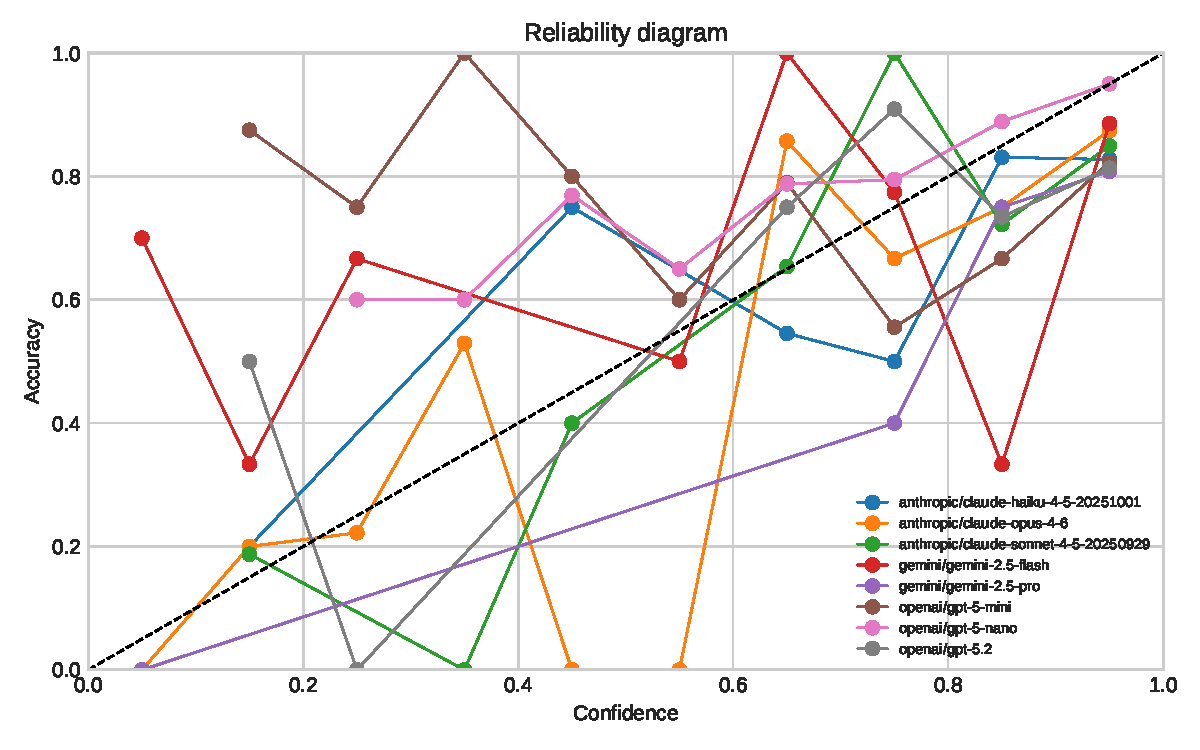
\includegraphics[width=0.98\linewidth]{figures/fig2_reliability_diagram_overlay.pdf}}{}
\caption{Overlaid reliability diagram (qualitative comparative view).}
\label{fig:reliability}
\end{figure}

\begin{figure}[t]
\centering
\IfFileExists{figures/fig3_mismatch_by_difficulty_bucket.pdf}{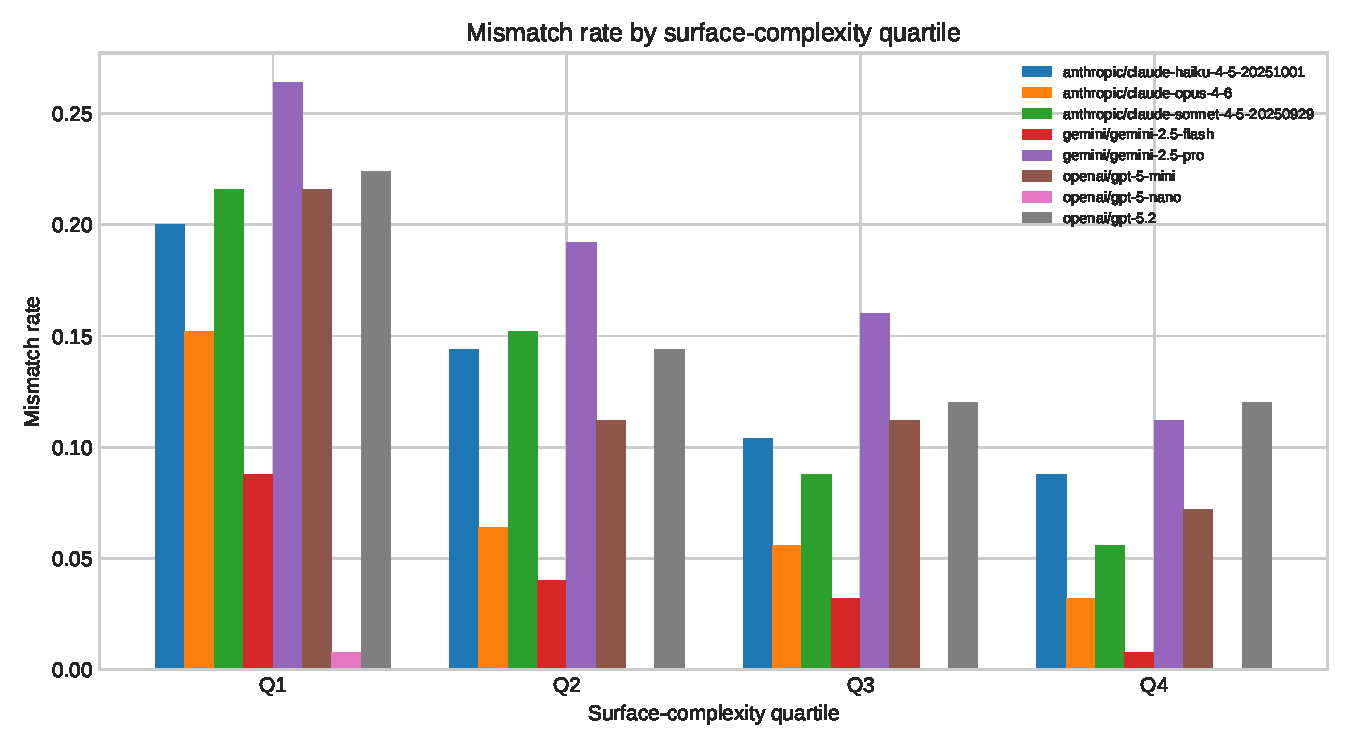
\includegraphics[width=0.98\linewidth]{figures/fig3_mismatch_by_difficulty_bucket.pdf}}{}
\caption{Mismatch@0.9 by source-side complexity quartile (secondary descriptive stratification).}
\label{fig:mismatch}
\end{figure}

\section{Trustworthiness Implications}
The evidence supports a narrow operational claim: self-reported confidence is useful only as a provider-local signal in this setup. Directly reusing the same threshold across providers risks inconsistent accepted-error behavior. For deployment, this points to provider-specific threshold tuning, explicit post-hoc calibration, or external evaluator layers instead of uncalibrated threshold sharing.

Supplementary artifacts show that isotonic remapping can reduce ECE for most providers, but mappings are provider-specific and do not restore portability.

\section{Limitations and Reproducibility Scope}
\textbf{Operational label, not semantic truth.} chrF-q20 is reproducible but not a semantic correctness label.

\textbf{Incomplete semantic and prompt robustness evidence.} The repository includes a semantic-audit scaffold, but no completed human labels. Prompt-variant infrastructure exists, but non-baseline outputs are not bundled.

\textbf{Metric packaging limits.} COMET/xCOMET checkpoints are not bundled; current offline robustness falls back to sentence BLEU where COMET is unavailable.

\textbf{Live API dependence for fresh raw runs.} Fully fresh generation requires provider credentials and is not self-contained offline.

\section{Conclusion}
Under a shared black-box protocol for English$\rightarrow$German MT, self-reported confidence is provider-dependent and non-portable as a common thresholding signal. For trustworthy decision support, confidence should be treated as a provider-specific control variable with explicit calibration and governance rather than a universal probability scale.

\bibliographystyle{plainnat}
\bibliography{references,added_refs}

\end{document}
